\documentclass{article}

\usepackage{amsmath}
\usepackage{amsfonts}
\usepackage{commath}
\usepackage[margin=1in]{geometry}
\usepackage{xfrac}
\usepackage{tkz-euclide}

\title{PHY202 Final Exam Portfolio}
\author{Nicolas Nytko}
\date{December 12, 2016}

\nonumber

\begin{document}
\maketitle
\newpage
\section{Polarization of Light}
When unpolarized light passes through a polarizer, the average intensity of the light will be half of the original intensity.
\[ I_1 = \frac{I_0}{2} \]
This light will now be polarized.  If it passes through another polarizer, the new intensity is dependent on the relative angle of the two polarizers.
\[ I_2 = I_1 \cos^2 \theta \]
This equation can be applied as many times as there are extra polarizers, just remember that $\theta$ is the angle between polarizer $n$ and $n-1$, not the angle that is made to the horizontal.
\section{Snell's Law and Total Internal Reflection}
\subsection{Law of Reflection}
When light is reflected off of a mirror, the angle of incidence and the angle of reflection are equal to each other.
\[ \theta_i = \theta_r \]
In this case, the angles are measured relative to the surface normal.
\subsection{Speed of Light}
As light enters different mediums, it will speed up or slow down based on the medium's index of refraction.  This new speed of light, $v$, can be found using the following proportionality:
\[v=\frac{c}{n}\]
Where $c$ is the speed of light in a vacuum, and $n$ is the medium's index of refraction.
\subsection{Snell's Law}
To find the refraction angle when light enters a new medium, Snell's law can be used.
\[n_1\sin\theta_1=n_2\sin\theta_2\]
Where $n_1$ is the first medium's index of refraction, $\theta_1$ is the angle of incidence relative to the normal, $n_2$ is the second medium's index, and $\theta_2$ is the angle of refraction relative to the normal.
\subsection{Critical Angle}
The critical angle is the maximum incidence angle that will still result in refraction.  To find this, set the refraction angle to be $\frac{\pi}{2}$, since anything larger will be outside of the medium, then solve for the incidence angle.
\begin{align*}
n_1\sin\theta_1&=n_2\sin\left(\frac{\pi}{2}\right) \\
\sin\theta_1&=\frac{n_2}{n_1} \\
\theta_1&=\sin^{-1}\left(\frac{n_2}{n_1}\right)
\end{align*}
Any angle of incidence larger than this critical angle will result in \textit{total internal reflection}.
\section{Ray Diagrams for Lenses and Mirrors}
The first step in drawing a ray diagram is to identify what type of mirror or lens needs to be drawn.  If it is a mirror, see if it curves towards or away the object.  If it curves towards, it is convex, if it curves away, it is concave.  If drawing a diagram for a lens, identify if it is converging or diverging.  Thin on top and bottom and thick in middle is converging, while thin in the middle and thick on top and bottom is diverging.  Draw the ray diagram according to what kind of lens or mirror it is.  The point where all of the rays intersect is the image position.
\subsection{Concave/Converging Mirrors}
Draw the object, mirror, focal points, and the inner center of radius point (twice the focal point). Starting from the top of the object, draw a ray parallel to the horizontal then reflecting through the focal point (P-Ray).  Draw a ray parallel to the focal point and reflecting parallel to the horizontal (F-Ray).  Draw the C-ray going through 
\newline
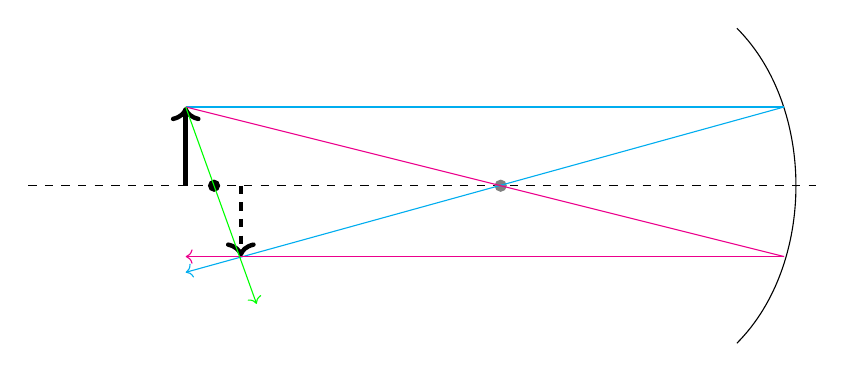
\begin{tikzpicture}
  \draw [dashed] (0,0) -- (10,0);
  \draw[ultra thick,->] (2,0) -- (2,1);
  \draw[ultra thick,dashed,->] (2.7,0) -- (2.7,-0.9);
  \draw (9,-2) .. controls(10,-1) and (10,1) .. (9,2);
  \filldraw[gray] (6,0) circle (2pt);
  \filldraw[black] (2.36,0) circle (2pt);
  \draw[cyan](2,1) -- (9.6,1);
  \draw[cyan,->](9.6,1) -- (2,-1.1);
  \draw[magenta](2,1) -- (9.6,-0.9);
  \draw[magenta,->](9.6,-0.9) -- (2,-0.9);
  \draw[green,->](2,1) -- (2.9,-1.5);
\end{tikzpicture}
\newline
In this image, the P-ray is blue, the F-ray is magenta, and the C-ray is green.
\subsection{Convex/Diverging Mirrors}
Draw the object, mirror, and focal point, this time the focal point is on the opposite side of the image.  Start from the top of the image and draw the F, P, and C-rays as before, except this time they also extend past the mirror to create a virtual image.  The C-ray goes through the outer C point.
\newline
\begin{tikzpicture}
  \draw [dashed] (0,0) -- (13,0);
  \draw[ultra thick,->] (2,0) -- (2,1);
  \draw[ultra thick,dashed,->] (6.9,0) -- (6.9,0.4);
  \draw (6,-2) .. controls(5,-1) and (5,1) .. (6,2);
  \filldraw[gray] (8,0) circle (2pt);
  \filldraw[black] (10.3,0) circle (2pt);
  \draw[cyan](2,1) -- (5.4,1);
  \draw[cyan,dashed](5.4,1) -- (8,0);
  \draw[cyan,->](5.4,1) -- (2.8,2);
  \draw[magenta](2,1)--(5.3,0.43);
  \draw[magenta,->](5.3,0.43)--(2.8,0.43);
  \draw[magenta,dashed,->](5.3,0.43) -- (8,0.43);
  \draw[green](2,1) -- (5.32,0.6);
  \draw[green,dashed](5.32,0.6) -- (10.3,0);
\end{tikzpicture}
\newline
In this image, the P-ray is blue, the F-ray is magenta, and the C-ray is green.
\subsection{Converging Lenses}
Draw the object, lens, and both focal points, which will be equidistant to the lens on both sides.  Draw the P-Ray parallel to the horizontal and then towards the outer focal point.  Draw the F-Ray towards the inner focal point then parallel to the horizontal when it reaches the lens.  Draw the C-Ray going throught the middle of the lens.
\newline
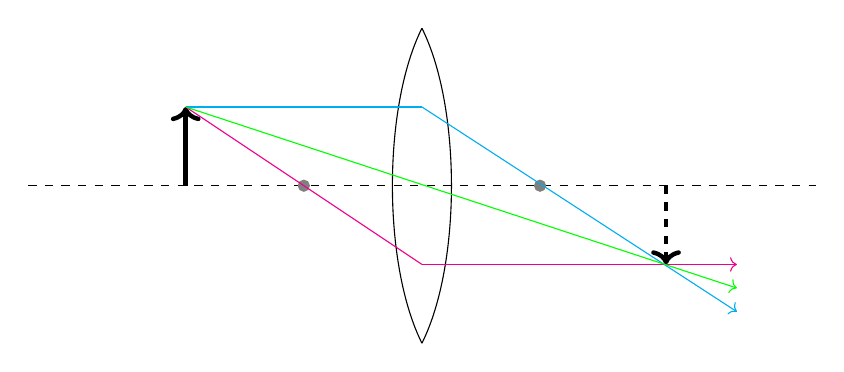
\begin{tikzpicture}
  \draw [dashed] (0,0) -- (10,0);
  \draw[ultra thick,->] (2,0) -- (2,1);
  \draw[ultra thick,dashed,->] (8.1,0) -- (8.1,-1);
  \draw (5,-2) .. controls(4.5,-1) and (4.5,1) .. (5,2);
  \draw (5,-2) .. controls(5.5,-1) and (5.5,1) .. (5,2);
  \filldraw[gray] (6.5,0) circle (2pt);
  \filldraw[gray] (3.5,0) circle (2pt);
  \draw[cyan](2,1) -- (5,1);
  \draw[cyan,->](5,1) -- (9,-1.6);
  \draw[magenta](2,1)--(5,-1);
  \draw[magenta,->](5,-1)--(9,-1);
  \draw[green,->](2,1)--(9,-1.3);
\end{tikzpicture}
\newline
In this image, the P-ray is blue, the F-ray is magenta, and the C-ray is green.
\subsection{Diverging Lenses}
Draw the object, lens, and focal points.  Draw the P-Ray parallel, then towards the inner focal point.  Draw the F-ray towards the outer focal point, then parallel.  Draw the C-Ray towards the center of the lens.  When the rays hit the lens, draw the resulting line in both directions in order to find the image.
\newline
\begin{tikzpicture}
  \draw [dashed] (0,0) -- (10,0);
  \draw[ultra thick,->] (2,0) -- (2,1);
  \draw[ultra thick,dashed,->] (4.4,0) -- (4.4,0.3);
  \draw (5,-2) .. controls(5.5,-1) and (5.5,1) .. (5,2);
  \draw (6,-2) .. controls(5.5,-1) and (5.5,1) .. (6,2);
  \draw(5,2) -- (6,2);
  \draw(5,-2) -- (6,-2);
  \filldraw[gray] (7,0) circle (2pt);
  \filldraw[gray] (4,0) circle (2pt);
  \draw[cyan](2,1) -- (5.5,1);
  \draw[cyan,dashed](5.5,1) -- (4,0);
  \draw[cyan,->](5.5,1) -- (7,2);
  \draw[magenta](2,1) -- (5.5,0.3);
  \draw[magenta,->](5.5,0.3) -- (7,0.3);
  \draw[magenta,dashed](5.5,0.3) -- (4,0.3);
  \draw[green,->](2,1)--(7,-0.45);
\end{tikzpicture}
\newline
In this image, the P-ray is blue, the F-ray is magenta, and the C-ray is green.
\section{Calculations for Single Lenses and Mirrors}
Given the radius of curvature of a lens or mirror, the focal point can be found by dividing it by two.
\[f=\frac{R}{2}\]
For a lens that has two different radii on its sides, the lens maker's equation can be used:
\[\frac{1}{f}=(n-1)\left(\frac{1}{R_1}+\frac{1}{R_2}\right)\]
The magnification of a lens or mirror, $M$, is given by the following equation:
\[M=\frac{h^\prime}{h}=-\frac{q}{p}\]
Where $h^\prime$ is the image height, $h$ is the object height, $q$ is the image distance, and $p$ is the object distance.  This equation can be used to find one of the distances when the other three are known.
\newline
The general equation for a lens or mirror is given by:
\[\frac{1}{f}=\frac{1}{p}+\frac{1}{q}\]
Where $f$ is the focal point, $p$ is object distance, and $q$ is the image distance.
\subsection{Sign Conventions}
Refer to this handy table for sign conventions:
\newline\newline
\begin{tabular}{|l l l|}
  \textbf{Quantity} & \textbf{Positive} & \textbf{Negative} \\
  Focal Point & Converging & Diverging \\
  Image Distance & Real & Virtual \\
  Image Height & Upright & Inverted
\end{tabular}
\section{Calculations for Double Lens Systems}
When dealing with double lens systems, first solve the first lens for the image height and distance.  This image becomes the object for the second distance.  To get the value of $p$ for the second lens, subtract the image distance from the distance between the two lenses.
\[p_2=d-q_1\]
The object height will be the same as the first image height because it is measured relative to the same horizontal axis.
\section{Interference Problems}
In an interference problem, it is important to remember the following variables:
\begin{itemize}
\item $d$, the distance between the slits in a double-slit
\item $D$, the size of the slit in a single slit
\item $y$, the distance from the center of the projection
\item $L$, the distance from the light projector to the screen
\item $\theta$, which is equal to $\tan^{-1}\left(\frac{y}{L}\right)$
\item $\phi$, the angle at which the waves of light are out of phase by in a double-slit at angle $\theta$
\end{itemize}
\subsection{Double Slit}
To find the bright spots in a double-slit interference problem, use the following equation:
\[d\sin\theta=m\lambda\]
Where $m$ is an integer greater than or equal to zero.
To find the dark spots in a double-slit, use this equation:
\[d\sin\theta=(m+\sfrac{1}{2})\lambda\]
To find the phase angle of the two light waves coming out of the slits at angle $\theta$, use this equation to find $\phi$:
\[\phi=\frac{2\pi}{\lambda}d\sin\theta\]
\subsection{Single Slit}
To find the dark spots in a single-slit interference problem, use this equation:
\[D\sin\theta=m\lambda\]
Where $m$ is an integer greater than or equal to one.
\subsection{Diffraction Grating}
If given the slit distance as a density, convert to meters and take the inverse to get $d$, the slit distance.
\[d=\frac{1}{\rho}\]
To find the bright spots, use the previously defined bright spot equation.
\[d\sin\theta=m\lambda\]
\end{document}